\begin{figure}
\caption{Forecast Errors}\label{fg:fe}\vspace*{1pc}
\begin{tabular}{ccc}
\multicolumn{3}{c}{Case 1: Rational Expectations} \\ 
Output Gap & Inflation & Fed Funds \\
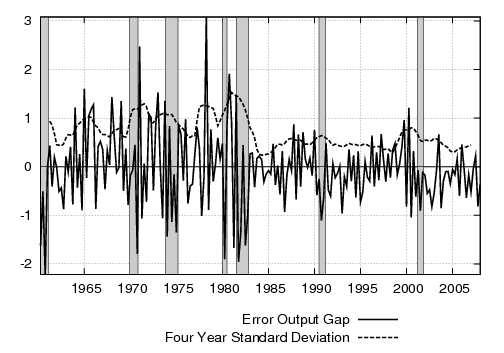
\includegraphics[scale=0.28]{results_re/output_err.png} & 
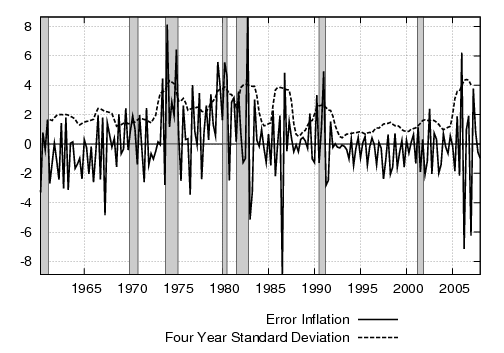
\includegraphics[scale=0.28]{results_re/inflation_err.png} & 
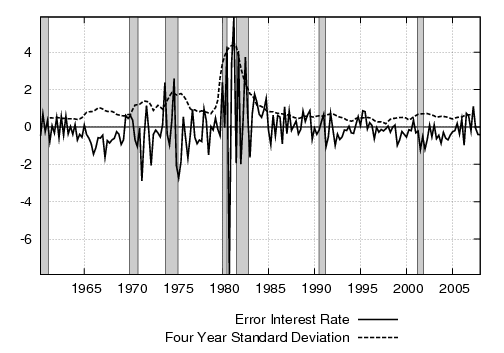
\includegraphics[scale=0.28]{results_re/fedfunds_err.png} \\ \\ 
 
\multicolumn{3}{c}{Case 2: Learing with RE Initial Conditions} \\ 
Output Gap (0.9724) & Inflation (0.9492) & Fed Funds (0.9525) \\
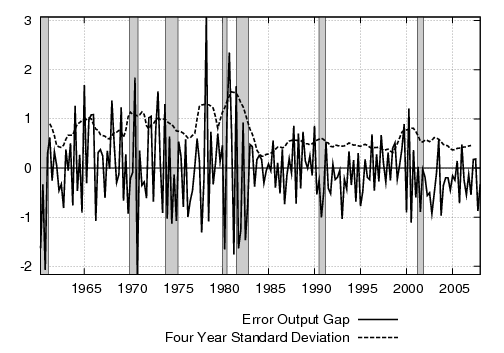
\includegraphics[scale=0.28]{results_reallinit/output_err.png} & 
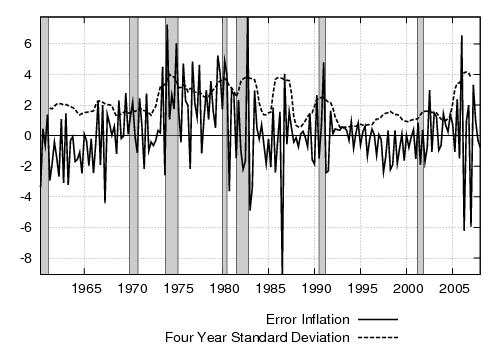
\includegraphics[scale=0.28]{results_reallinit/inflation_err.png} & 
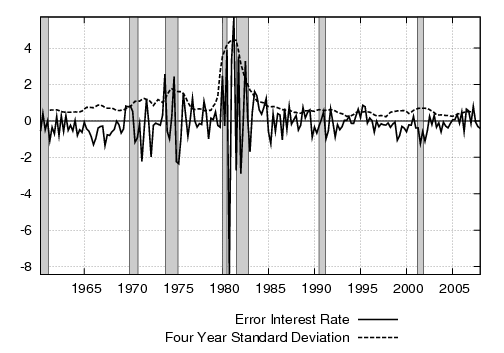
\includegraphics[scale=0.28]{results_reallinit/fedfunds_err.png} \\ \\ 
 
\multicolumn{3}{c}{Case 3: Learing with RE Initial Conditions, Shocks Unobservable} \\ 
Output Gap (0.9329) & Inflation (0.9474) & Fed Funds (0.9461) \\
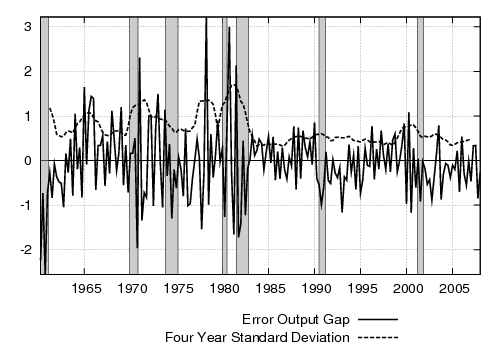
\includegraphics[scale=0.28]{results_reinit/output_err.png} & 
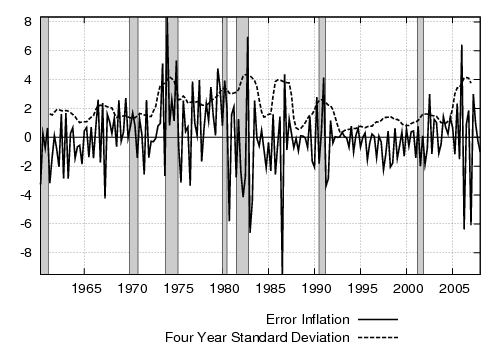
\includegraphics[scale=0.28]{results_reinit/inflation_err.png} & 
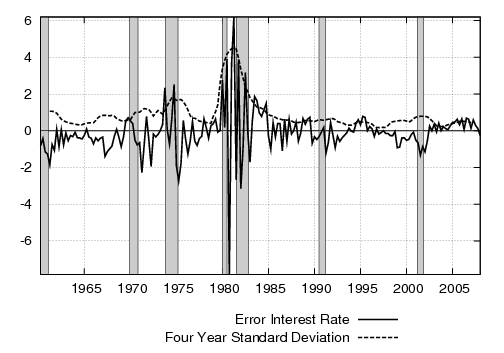
\includegraphics[scale=0.28]{results_reinit/fedfunds_err.png} \\ \\ 
 
\multicolumn{3}{c}{Case 4: Learning with Unobservable Shocks and Pre-Sample Initial Conditions} \\ 
Output Gap (0.9219) & Inflation (0.9121) & Fed Funds (0.9586) \\
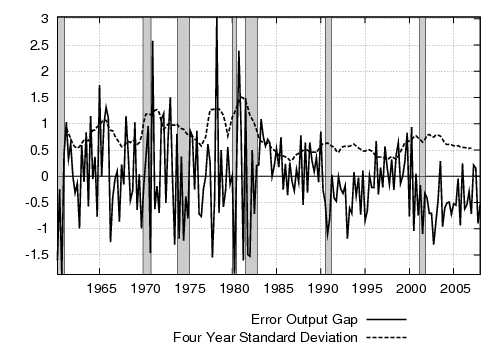
\includegraphics[scale=0.28]{results_wlsinit/output_err.png} & 
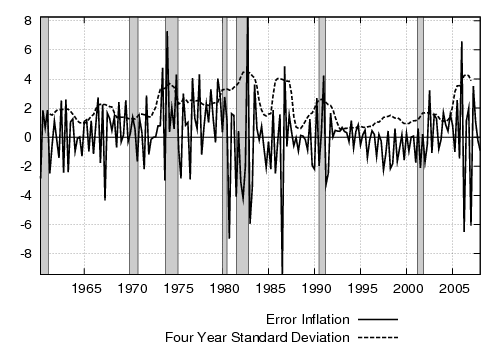
\includegraphics[scale=0.28]{results_wlsinit/inflation_err.png} & 
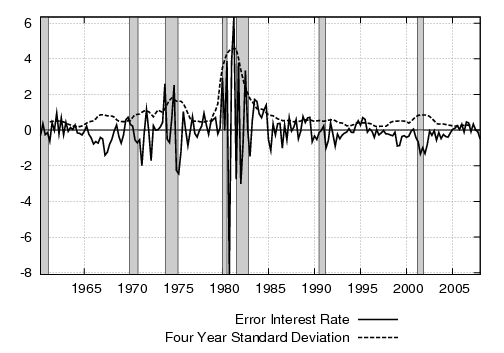
\includegraphics[scale=0.28]{results_wlsinit/fedfunds_err.png} \\ \\ 
 
\end{tabular}
\end{figure}
